\graphicspath{{images/}}

\section*{Turingmaschinen}

\begin{theorem}{Turingmaschine (TM)} $M=\left(Q, \Sigma, \Gamma, \delta, q_{0}, \sqcup , F\right)$

    \begin{minipage}{0.45\linewidth}
        $Q$: Menge von Zuständen

        $\Sigma$: Alphabet der Eingabe

        $\Gamma$ und $\Sigma \subset \Gamma$: Bandalphabet
    \end{minipage}
    \begin{minipage}{0.55\linewidth}
        $q_{0} \in Q$: Anfangszustand

        $F \subseteq Q$: Akzeptierende Zustände

        ${ }_{\sqcup }$: Leerzeichen mit ${ }_{\mu} \in \Gamma$ und ${ }_{\mu} \notin \Sigma$
    \end{minipage}

    Übergangsfunktion: $\boldsymbol{\delta}: \boldsymbol{Q} \times \boldsymbol{\Gamma} \rightarrow \boldsymbol{Q} \times \boldsymbol{\Gamma} \times \boldsymbol{D}, \boldsymbol{D}=\{\boldsymbol{L}, \boldsymbol{R}\}$
    
    \vspace{1mm}

    Sie bestehen aus einem Lese-/Schreibkopf und einem unendlichen Band von Zellen.

    \vspace{1mm}

    Sie bildet das 2-Tupel $(q, X)$ auf das Tripel $(p, Y, D)$

    \begin{minipage}{0.45\linewidth}
        $D=$ Direction

        $X=$ Read

        $Y=$ Overwrite
    \end{minipage}
    \begin{minipage}{0.5\linewidth}
       $q, p \in Q$ und $X, Y \in \Gamma$

       \vspace{1mm}

       \emph{$q-X / Y, D \rightarrow p$}
    \end{minipage}

    \vspace{1mm}
    {\small Wenn TM anhält, dann fertig (akzeptierend falls in $F$). Resultat = Bandinhalt}
\end{theorem}

\begin{definition}{Band} 
    Zellen mit je 1 Symbol, Anfangszustand: enthält Eingabe (endliches Wort aus $\Sigma^{*}$), alle anderen Zellen: $\sqcup$
\end{definition}

\begin{definition}{Konfiguration einer TM}
    Zustand der Zustandssteuerung, Position des Lese-/Schreibkopfes und Bandinhalt
\end{definition}

\begin{example2}{Universelle TM} Codierung der Übergangsfunktion (Gödelnummer)

    \begin{minipage}{0.45\linewidth}
        \textcolor{green}{Zustände} $q_n := 0^n$\\
        \textcolor{blue}{Symbole} $\Gamma = \{0, 1, \$, a \in \Sigma\}$\\ (0 = 0, 1 = 00, \$ = 000)\\
        \textcolor{orange}{Richtung} L = 0, R = 00
    \end{minipage}
    \begin{minipage}{0.55\linewidth}
    \textcolor{pink}{Trennzeichen}
    \begin{itemize}
        \item zwischen Elementen: 1
        \item zwischen Übergangsfunktionen: 11
        \item Ende der Turingmaschine: 111\\ danach \textcolor{purple}{Input}
    \end{itemize}  
    \end{minipage}

    \vspace{1mm}

    bsp: \textcolor{green}{0}\textcolor{pink}{1}\textcolor{blue}{00}\textcolor{pink}{1}\textcolor{green}{00}\textcolor{pink}{1}\textcolor{blue}{0}\textcolor{pink}{1}\textcolor{orange}{00}\textcolor{pink}{00}\textcolor{green}{000}\textcolor{pink}{1}...\textcolor{blue}{0}\textcolor{pink}{1}\textcolor{orange}{1}\textcolor{pink}{111}\textcolor{purple}{1101...}
\end{example2}

\begin{remark}
    Alle Arten von TMs gleichmächtig, da jede TM durch eine DTM simuliert werden kann.
\end{remark}

\begin{example2}{Mehrband-Maschine}\\
    \begin{minipage}{0.4\linewidth}
    Spezifizieren Sie eine TM $M_{4}$, welche die Subtraktion von zwei natürlichen Zahlen $(a-b$, mit $a \geq b)$ realisiert.
    \end{minipage}
    \begin{minipage}{0.6\linewidth}
        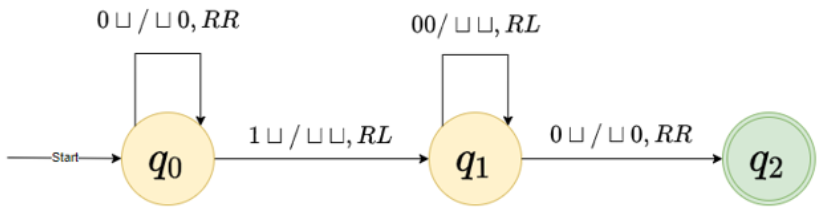
\includegraphics[width=1\linewidth]{images/mehrband_maschine1.png}
    \end{minipage}
    
    Beispiel: $4-2=2$\\
    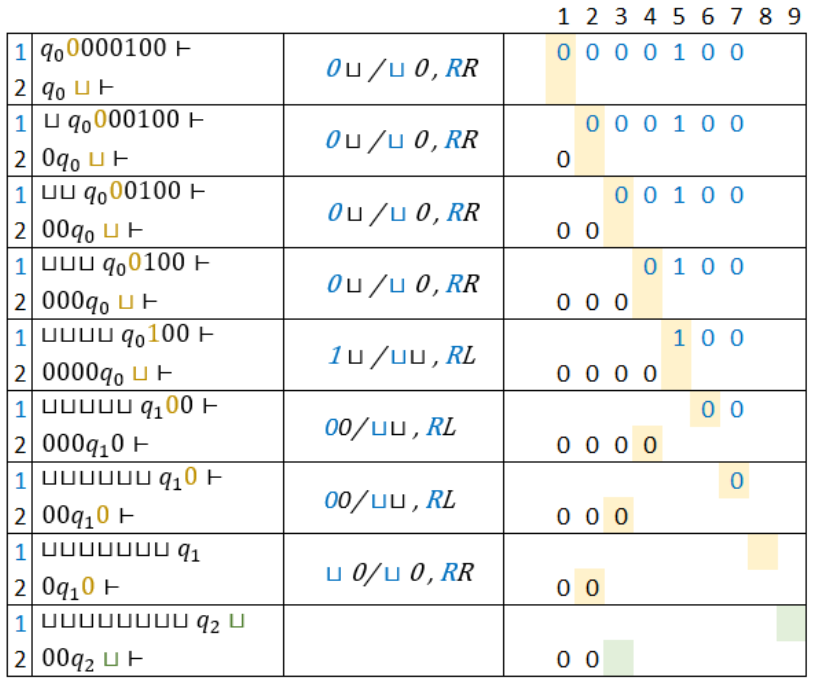
\includegraphics[width=0.7\linewidth]{images/mehrband_maschine2.png}
\end{example2}


